% Hero figure: a real scan, its **kern output, and test-set error.
% Scan: Liszt, Hungarian Rhapsody No. 2, IMSLP file 300584, page 26
% (public domain), system 1 of the 1050 px model input.
% Code: first lines of Transcoda + CD output for this page, converted to Humdrum.
% Bars: mean OMR-NED from evaluation/ (frozen summaries and baseline reports).
\documentclass[border=6pt]{standalone}
% Shared preamble for the README figures. Compile with build.sh.
\usepackage[T1]{fontenc}
\usepackage[sfdefault,scale=0.95,lining]{FiraSans}
\usepackage[scale=0.9]{sourcecodepro}
\usepackage{textcomp}
\usepackage{graphicx}
\usepackage{xcolor}
\usepackage{tikz}
\usepackage{pgfplots}
\pgfplotsset{compat=1.18}
\usetikzlibrary{arrows.meta,positioning,calc,backgrounds,fit,decorations.pathreplacing}
\graphicspath{{assets/}}
\definecolor{ink}{HTML}{1F2328}
\definecolor{muted}{HTML}{59636E}
\definecolor{rule}{HTML}{D1D9E0}
\definecolor{codebg}{HTML}{F6F8FA}
\definecolor{tc}{HTML}{6F42C1}
\definecolor{tclight}{HTML}{C9B6F2}
\definecolor{legato}{HTML}{F0A35E}
\definecolor{smt}{HTML}{9DB4D6}
\color{ink}

\begin{document}
\begin{tikzpicture}[
    lab/.style={font=\small\bfseries, text=muted, anchor=south west, inner sep=0pt},
    arr/.style={-{Stealth[length=7pt,width=7pt]}, line width=1.4pt, tc},
]
% Left column: scan -> model -> **kern
\node[lab] at (0,8.55) {REAL SCAN \textmd{(IMSLP, public domain)}};
\node[anchor=north west, inner sep=0pt] (scan) at (0,8.35)
    {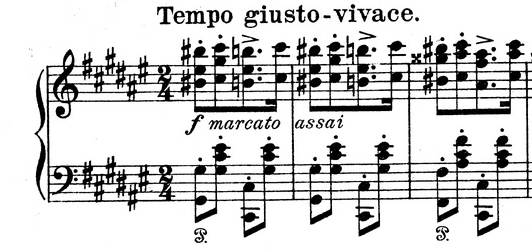
\includegraphics[width=7.9cm]{liszt-p26-system1.png}};
\node[fill=tc, text=white, rounded corners=8pt, font=\small\bfseries, inner xsep=9pt, inner ysep=4pt]
    (model) at ($(scan.south)+(0,-0.72)$) {Transcoda};
\draw[arr] (scan.south) -- (model.north);
\node[anchor=north, font=\ttfamily\small, align=left, fill=codebg, draw=rule, line width=0.6pt,
      rounded corners=3pt, inner xsep=9pt, inner ysep=7pt, text width=7.26cm] (code) at ($(model.south)+(0,-0.42)$) {%
\begin{tabular}{@{}l@{\hspace{2.2em}}l@{}}
\textcolor{tc}{**kern}     & \textcolor{tc}{**kern}\\
{*}clefF4                  & {*}clefG2\\
{*}k[f\#c\#g\#d\#a\#e\#]   & {*}k[f\#c\#g\#d\#a\#e\#]\\
{*}M2/4                    & {*}M2/4\\
8GG\# 8G\#L                & 8b\# 8ee\# 8bbL\\
8G\# 8c\# 8e\#J            & 8cc\# 8gg\# 8ccc\#\\
8CC\# 8C\#L                & 8.b 8.ee\# 8.bb\\
\textcolor{muted}{\dots}   & \textcolor{muted}{\dots}
\end{tabular}};
\draw[arr] (model.south) -- (code.north);
% Right column: OMR-NED bars
\node[lab] at (9.0,8.55) {TEST ERROR \textmd{(OMR-NED \%, lower is better)}};
\begin{axis}[
    at={(9.75cm,0.62cm)}, anchor=south west,
    width=7.9cm, height=5.9cm, scale only axis,
    /pgf/number format/assume math mode=true,
    ybar, bar width=19pt,
    ymin=0, ymax=112, ytick={0,25,50,75,100},
    axis line style={rule}, tick style={draw=none},
    ymajorgrids, grid style={rule, line width=0.4pt},
    axis x line*=bottom, axis y line*=left,
    tick label style={font=\small, text=muted},
    symbolic x coords={syn,real}, xtick=data, enlarge x limits=0.4,
    xticklabels={{Synthetic test\\[-1pt]\footnotesize 2,500 pages}, {IMSLP-Real\\[-1pt]\footnotesize 202 real scans}},
    xticklabel style={align=center, font=\small, text=ink},
    nodes near coords, every node near coord/.append style={font=\footnotesize\bfseries, text=ink, inner sep=2pt,
        /pgf/number format/.cd, fixed, fixed zerofill, precision=2},
    legend style={at={(0.5,1.04)}, anchor=south, legend columns=2, draw=none, fill=none,
        font=\small, /tikz/every even column/.append style={column sep=12pt}},
    legend cell align=left,
    legend image code/.code={\fill[#1] (0cm,-0.09cm) rectangle (0.3cm,0.13cm);},
]
\addplot[fill=smt, draw=none]     coordinates {(syn,94.97) (real,97.41)};
\addplot[fill=legato, draw=none]  coordinates {(syn,18.61) (real,53.20)};
\addplot[fill=tclight, draw=none] coordinates {(syn,1.56)  (real,28.50)};
\addplot[fill=tc, draw=none]      coordinates {(syn,1.25)  (real,22.59)};
\legend{SMT++, Legato, Transcoda (beam), Transcoda + CD}
\end{axis}
\end{tikzpicture}
\end{document}
